%%%%%%%%%%%%%%%%%%%%%%%%%%%%%%%%%%%%%%%%%%%%%%%%%%%%%%%%%%%%%%%%%%%%%%%%
%                                                                      %
%     File: Thesis_Implementation.tex                                  %
%     Tex Master: Thesis.tex                                           %
%                                                                      %
%     Author: Andre C. Marta                                           %
%     Last modified : 13 May 2019                                      %
%                                                                      %
%%%%%%%%%%%%%%%%%%%%%%%%%%%%%%%%%%%%%%%%%%%%%%%%%%%%%%%%%%%%%%%%%%%%%%%%



\chapter{Fundamentos de um switch}
\label{chapter:implementation}
\section{LAN e MAC \textit{bridge}}
A Ethernet foi introduzida em 1973 pelo grupo de trabalho IEEE 802.3 com o propósito de interligar computadores e outros dispositivos em redes de área local (LAN). LAN são redes que interconectam computadores numa área limitada como um campus ou um escritório. Nestas, os vários dispositivos têm um endereço físico que deve ser único na rede, denominado de endereço MAC. \par 
Um dispositivo genericamente denominado de \textit{bridge} é usado para agregar segmentos de uma LAN ou um conjunto de LANs. As regras que devem ser seguidas pelas \textit{bridges} foram definidas na norma IEEE 802.1D  \cite{Bridge}. As \textit{bridges} possuem o mínimo de dois pontos de acesso a canais de comunicação da rede, denominados de portos, e reencaminham pacotes de informação entre os mesmos. A estes pacotes chama-se tramas e o seu formato varia consoante a tecnologia em que esteja implementada a LAN. \par 
As \textit{bridges} possuem uma tabela que faz a associação entre os vários endereços MAC do seu conhecimento e os portos das mesmas que estão interligados com o dispositivo com o respectivo endereço. No momento de receção de uma trama, a \textit{bridge} faz uma procura pelo endereço MAC de destino presente no cabeçalho da trama. Se o endereço for encontrado e o porto associado não coincidir com o porto de receção da trama, a mesma é transmitida para o porto associado, denominando-se de envio \textit{unicast}. Contrariamente, se o endereço não for encontrado, a trama é enviada por todos os restantes portos, denominando-se o envio de \textit{broadcast}. Por sua vez, o endereço de origem presente no cabeçalho pode ser adicionado à tabela juntamente com o porto de receção.

\par Na figura 3.1 está ilustrada uma LAN com 8 computadores e uma \textit{bridge} juntamente com o preenchemento da tabela de endereços do mesmo.



\begin{figure}[H]
  \centering
  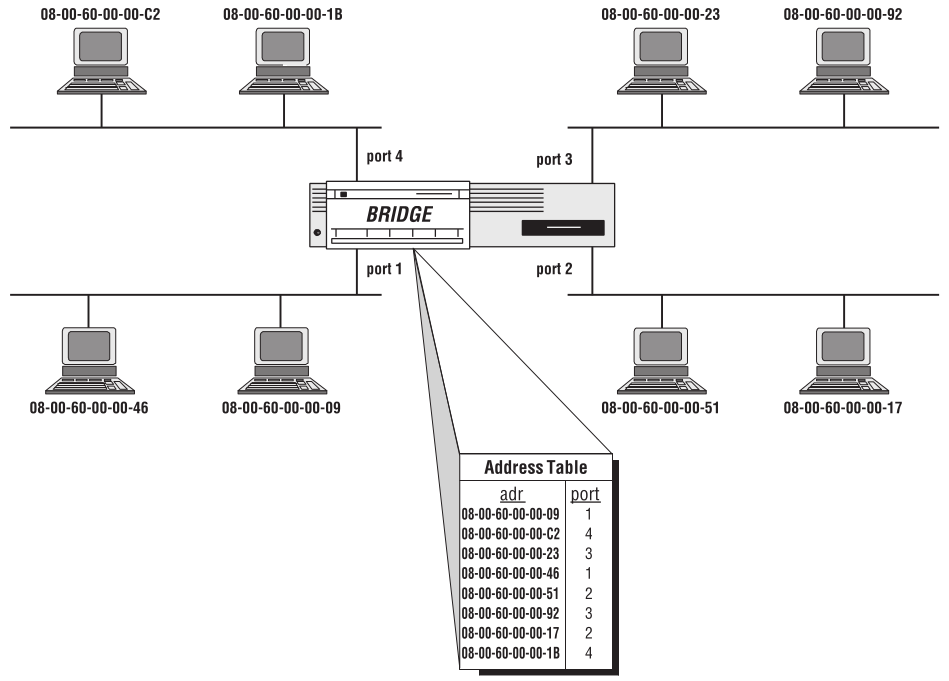
\includegraphics[width=1\textwidth]{Bridge.png}
  \caption[MAC bridge]{MAC \textit{bridge} \cite{make}}
  \label{fig:airbus1}
\end{figure}

\subsection{LAN virtual}

Na norma IEEE 802.1Q foi introduzido o conceito de LAN virtual (VLAN). Estas consistem numa divisão de uma rede fisicamente interligada num conjunto de LANs logicamente separadas. Numa VLAN, os seus membros apenas trocam informação com outros membros da mesma VLAN ainda que possa haver caminhos disponíveis para comunicar com membros de outras VLANs. As VLAN permitem aumentar a escalabilidade de uma rede, facilitar a mobilidade dos elementos da rede, aumentar a segurança e diminuir o tráfego desnecessário na mesma. \par

A sepração da rede em VLAN é implementada com recurso a switches com a capacidade de identificar a VLAN a que uma trama pertence e de usar essa informação na decisão do reencaminhamento da trama. A identificação da VLAN a que a trama pertence é efectuada com recurso à etiqueta VLAN que pode estar incluíada na trama. Esta tem a dimensão de dois octetos e está dividida nos seguintes 4 campos:

\begin{itemize}
  \item \textit{Tag Protocol Identifier}  - \quad Um código com a dimensão de um octeto que sinaliza a inclusão da etiqueta na trama.
  \item \textit{Priority Code Point}  - \quad Três bits que indicam a prioridade de transmissão da trama. Este campo não está diretamente associado à gestão das VLAN vai foi inserido na etiqueta por conveniência.
  \item \textit{Drop Eligeble Indicator}  - \quad Um bit que dá indicação de se a trama pode ser descartada em caso de congestionamento. Tal como o campo anterior foi inserido na etiqueta por conveniência.
  \item VLAN \textit{Identifier}  - \quad Identificador da VLAN à qual a trama pertence com a dimensão de doze bits. 
  \end{itemize}

  Quando a etiqueta não vem incluída na trama o switch pode identificar a VLAN a que esta pertence com recurso a diferentes estratégias. A mais comum e apoiada pela norma IEEE 802.1Q é a associação por porto. Nesta o switch mantém uma lista de da VLAN a que conecta cada um dos seus portos. 
  Um exemplo da associação de VLAN a portos está ilustrada na figura 3.2

  
\begin{figure}[H]
  \centering
  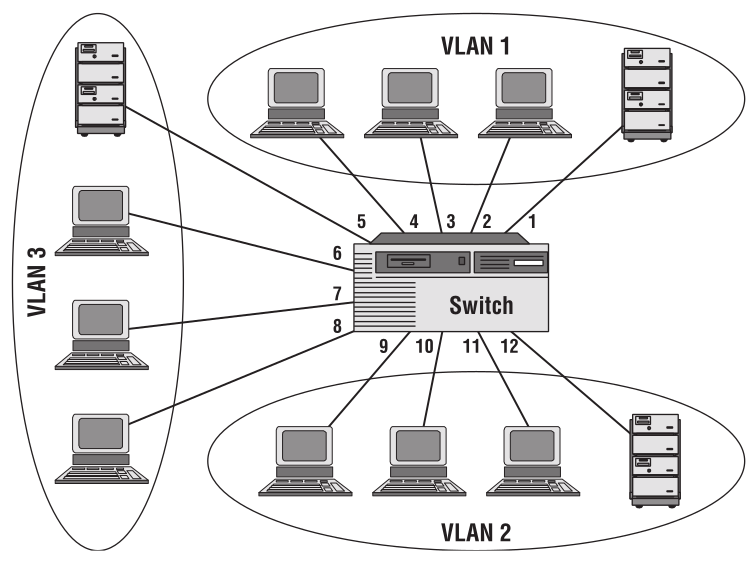
\includegraphics[width=0.7\textwidth]{Port_ASS.png}
  \caption[Associação porto-VLAN]{Associação porto-VLAN}
  \label{fig:airbus1}
\end{figure}

A tabela a consultar no momento da receção da trama para identificação da VLAN corrrespondente pode ser preenchida estaticamente ou dinamicamente com recurso a protocolos como o GARP. \par




\subsection{\textit{Spanning tree protocol}}


\section{\textit{Ethernet}}
\label{section:model}
 A Ethernet foi introduzida em 1973 pelo grupo de trabalho IEEE 802.3 com vista à sua utilização em redes LAN. Devido à sua simplicidade, baixo-custo e padronização de implementação, ganhou preponderância globalmente e foi a sua utilização foi extendida a redes de mais vasta área geográfica. Na atualidade, a maioria do tráfego da internet é gerado a partir de redes \textit{Ethernet}. Na sua versão primordial, a \textit{Ethernet} tinha débitos de 10 Mbps em ligações \textit{half-duplex}, sobre uma topologia \textit{bus} com o dispositivo conhecido como Ethernet \textit{Hub} a funcionar como \textit{bridge}. Tal significava que vários dispositivos partilhavam um único canal de comunicação, tendo que dividir o débito do canal entre si. De forma a gerenciar os acessos ao canal, implementava-se o mecanismo \textit{carrier-sense multiple access}. Posteriormente, com o aparecimento de tecnologias com maior débito como \textit{Fast Ethernet} e \textit{Gigabit Ethernet}, os \textit{Ethernet Hubs} foram substituídos por switches e as ligações \textit{half-duplex} por ligações \textit{full-duplex} segundo uma topologia em estrela, ganhando a designação comum de \textit{Switch-Ethernet}, devido à centralidade do referido dispositivo no funcionamento da rede. \par 
 
 \subsection{Trama de Ethernet}
 
Atualmente existem alguns tipos de tramas diferentes, divididas em vários campos de dados, consoante a norma aplicável. A versão mais predominante é a \textit{Ethernet} II. Nesta versão, os vários campos das tramas, as suas regras e conteúdo são os seguintes: 

\begin{itemize}
  \item Preâmbulo  - \quad Não pertence diretamente à trama, servindo como sinal para que o dispositivo que a recebe sincronize o seu ciclo de relógio ao canal de transmissão. É constituído por sete bytes consecutivos com o valor 10101010. 
  \item \textit{Start Frame Delimiter} (SFD)  - \quad Tal como o preâmbulo, não pertence diretamente à trama, sendo usado para sinalizar o início do envio da trama. É constituído por um byte com o valor 10101011.  
  \item Origem  - \quad Campo com a dimensão de 6 bytes, portador do endereço MAC do dispositivo que iniciou o envio da trama.
  \item Destino - \quad Campo com a dimensão de 6 bytes, portador do endereço MAC do dispositivo ao qual se destina a trama.
  \item IEEE 802.1Q -\quad Etiqueta VLAN explicada previamente que pode ser incluída na trama.
  \item \textit{EtherType} - \quad Campo que transmite a informação relativa ao campo de dados da trama. O valor deste campo deve ser superior a 1536, e indica o protocolo de mais alto nível que encapsula o campo de dados. No caso do PTP este campo tem o valor 0x88F7. Noutras normas, como o IEEE 802.3, este campo pode ter um valor inferior a 1500 e transmite o comprimento do campo de dados.
  \item \textit{Payload} - \quad Campo que contém os dados a serem transmitidos na rede. No caso do PTP, o cabeçalho, corpo e, quando existam, TLVs de uma mensagem são inseridos no \textit{Payload} da trama.
  \item \textit{Frame Check Sequence} (FCS). -\quad Campo que contém os 4 bytes de um código gerado pelo último dispositivo que manipulou a trama e afixado no final da mesma. No dispositivo que recebe a trama e nos switches que a retransmitem, o código é calculado novamente, e caso não coincida com o FCS incluido na trama, significa que esta sofreu erros. O FCS pode ser gerado de várias formas, mas tipicamente consiste num \textit{Cyclic Redundant Check} (CRC). 

  

\begin{figure}[H]
  \centering
  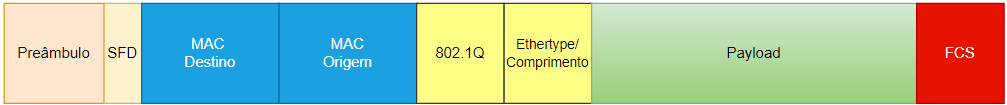
\includegraphics[width=1.\textwidth]{trama_best.png}
  \caption[Trama de Ethernet]{Formato de uma trama}
  \label{fig:airbus1}
\end{figure}


  
\end{itemize}


\subsection{\textit{Cyclic Redundancy Check}}


A norma IEEE 802.1D impôe a implementação de uma mecanismo de verificação de erros em tramas, ou seja, o FCS previamente mencionado. Em Ethernet é usado um \textit{Cyclic Redundant Check} (CRC). Este faz parte da classe de código cíclicos. O CRC é calculado pelo dispositivo que gera a trama e inserido no campo FCS. Aquando da receção da trama noutro disposito, o CRC deve ser novamente calculado. Quando CRC calculado coincide com o que vem na trama é considerado que esta está ausente de erros. Contrariamente, caso não coincidam, a norma IEEE 802.1D impõe que a trama seja descartada devido a provavel presença de erros na mesma.\par
O código CRC é o resto da divisão módulo 2 da trama acrescida de 4 octetos nulos por um polinómio de grau 32 sobre um campo finito de dois elementos. Devido à propriedade de as subtrações serem iguais às somas em campos finitos de dois elementos, a adição do CRC à trama garante que esta passa a ser divisível pelo polinómio gerador do CRC. Daí resulta que calcular o CRC da totalidade de uma trama recebida num dispositivo deve produzir 32 bits com o valor 0.\par
A divisão de dois polinómio em campos finitos de dois elementos pode ser efectuada iterativamente através da subtração de múltiplos do divisor sobre o dividendo. As subtrações, por sua vez, são iguais ás somas. Seguidamente são detalhados as etapas a efectuar numa iteração da divisão. 

\begin{enumerate}
\item Multiplicar o divisor por \(x^{n}\). O índice n na primeira iteração é igual à diferença entre o expoente máximo do dividendo e o expoente máximo do divisor.
\item Subtrair o dividendo pelo produto do divisor por \(x^{n}\).
\item Se n igual a 0, finalizar o algoritmo. Caso contrário, decrementar n.
\end{enumerate}

Na tabela 3.1 é dado o exemplo da divisão do polinómio \(x^{9} + x^{8} + x^{7} + x^{6} + x^{5}\) por \(x^{3} + x^{1}\) com o algoritmo descrito.


\begin{table}[H]
\begin{center} 
\begin{tabular}{|l l l l l l l l l l|}

    \hline
    \rowcolor{lightgray}
    1 & 1 & 1 & 1 & 1 & 0 & 0 & 0 & 0 & 0 \\
    \cellcolor{green}1 & \cellcolor{green}0 & \cellcolor{green}1 & \cellcolor{green}0 & & & & & & \\
    \hline
    \rowcolor{lightgray}
    0 & 1 & 0 & 1 & 1 & 0 & 0 & 0 & 0 & 0 \\
    & \cellcolor{green}1 & \cellcolor{green}0 & \cellcolor{green}1 & \cellcolor{green}0 & & & & &\\
    \hline
    \rowcolor{lightgray}
    0 & 0 & 0 & 0 & 1 & 0 & 0 & 0 & 0 & 0 \\
    & & \cellcolor{red}1 & \cellcolor{red}0 & \cellcolor{red}1 & \cellcolor{red}0 & & & & \\
    \hline
    \rowcolor{lightgray}
    0 & 0 & 0 & 0 & 1 & 0 & 0 & 0 & 0 & 0 \\
    & & & \cellcolor{red}1 & \cellcolor{red}0 & \cellcolor{red}1 & \cellcolor{red}0 & & & \\
    \hline
    \rowcolor{lightgray}
    0 & 0 & 0 & 0 & 1 & 0 & 0 & 0 & 0 & 0 \\
    & & & & \cellcolor{green}1 & \cellcolor{green}0 & \cellcolor{green}1 & \cellcolor{green}0 & & \\
    \hline
    \rowcolor{lightgray}
    0 & 0 & 0 & 0 & 0 & 0 & 1 & 0 & 0 & 0 \\
    & & & & & \cellcolor{red}1 & \cellcolor{red}0 & \cellcolor{red}1 & \cellcolor{red}0 & \\
    \hline
    \rowcolor{lightgray}
    0 & 0 & 0 & 0 & 0 & 0 & 1 & 0 & 0 & 0 \\
    & & & & & & \cellcolor{green}1 & \cellcolor{green}0 & \cellcolor{green}1 & \cellcolor{green}0 \\
    \hline
    \cellcolor{lightgray}0 & \cellcolor{lightgray}0 & \cellcolor{lightgray}0 & \cellcolor{lightgray}0 & \cellcolor{lightgray}0 & \cellcolor{lightgray}0 & \cellcolor{blue}0 & \cellcolor{blue}0 & \cellcolor{blue}1 & \cellcolor{blue}0 \\
    \hline
    
\end{tabular}
\end{center}

\end{table}


Na primeira iteração do processo de divisão o divisor é multiplicador por \(x^{6}\) resultando no polinómio \(x^{9} + x^{7}\). Por sua vez, ese resultado é subtraido no dividendo obtendo-se o polinómio \(x^{8} + x^{6} + x^{5}\) que é usado como dividendo na seguinte iteração. No final do algoritmo é obtido, como resto da divisão, o polinómio \(x^{1}\) que pode ser representado binariamente como 010. \par
O algoritmo demonstrado é de fácil implementação em RTL, o que contribuiu para a utilização do CRC como método de deteção de erros em Ethernet.  



\section{Componentes}
\label{section:model}

O switch de \textit{Ethernet} é uma classe de dispositivos de elevada complexidade. Um switch além de receber e enviar tramas, deve também ser capaz de aprender enquanto membro de uma rede, quais os portos que levam as tramas a chegar aos destinos desejados, verificar a ocorrência de erros, seguir as regras de VLAN, proceder ao processamento, criação e alteração de tramas segundo protocolos de alto nível e, como é o caso no PTP, participar ativamente na execução dos protocolos. Para isso, as arquitecturas dos switches são divididas em vários módulos, cada qual responsável por executar uma tarefa específica dentro das várias necessárias no dispositivo. Alguns módulos podem estar ou não presentes e seguir abordagens distintas consoante as arquitecturas que sejam escolhidas na utilização que se pretende para o switch. No entanto, alguns componentes são fundamentais e devem servir como base no desenvolvimento de um switch. Dois desses componentes vitais a um switch são a tabela de endereços e a \textit{switch fabric} \cite{make}. \par
\subsection{Lógica de reencaminhamento}
A procura, inserção e eliminação de elementos da tabela pode ser implementada com diferentes abordagens, variando em eficácia, eficiência temporal, eficiência de utilização de memória, quantidade de \textit{hardware} necessário e complexidade no desenvolvimento e, em última análise, em custo monetário. As duas formas mais comuns de implementar o processamento da tabela é com recurso a algoritmos de procura semelhantes aos usados em \textit{software}, ou, quando possível, com recurso a memórias CAM (\textit{Content Addressable Memory}) \cite{CAM}. As memórias CAM são um tipo de memória muito usado em redes de computadores e em aplicações que exijam uma elevada eficiência temporal. O seu modo de operação consiste em serem capazes de devolver o endereço de memória de um conjunto de bits que estejam armazenados na mesma em apenas um ciclo de relógio. Para o conseguirem, as células de uma memória CAM, que armazenam um bit de informação, têm um circuito semelhante ao de uma célula SRAM, à qual são adicionados quatro transístores para funcionarem como comparadores entre o conteúdo de uma célula e os bits de uma palavra que se procura na CAM. O circuito básico pode ser observado na figura 3.3. Os transístores M1, M2, M3 e M4 são responsáveis pela comparação entre D, o bit armazenado, e SL, o bit da palavra. O par de transístores M1 e M3, tal como o par M2 e M4 funcionam como um caminho entre ML e a terra. Quando SL e D têm valores opostos, ou seja, o bit que se procura difere do bit armazenado, um dos dois caminhos conduz corrente forçando ML a ficar com a tensão de terra. Contrariamente, se houver correspondência entre D e SL, os caminhos não conduzem, desconectando ML da terra.  Quando ML é desconectado em todas as células que armazenam os bits de uma palavra, um sinal com o valor lógico 1 é introduzido num codificador levando a que a saída do mesmo seja o endereço de memória da palavra que se procurava. Um exemplo de uma \textit{CAM} que armazena palavras de 3 bits pode ser observado na figura 3.2.

\begin{figure}[H]
\centering
\begin{minipage}{.5\textwidth}
  \centering
  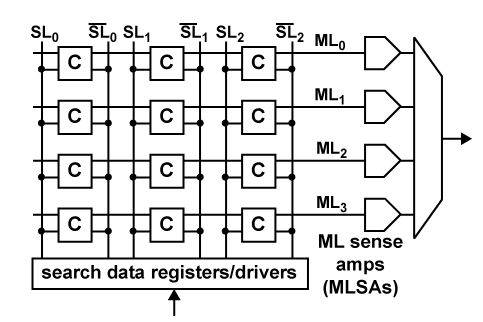
\includegraphics[width=.9\linewidth]{CAM_TOP.png}
  \caption{Memória CAM}{(fonte: \cite{CAM})}
  \label{fig:test1}
\end{minipage}%
\begin{minipage}{.5\textwidth}
  \centering
  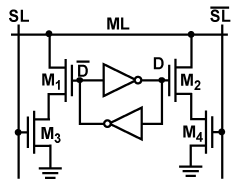
\includegraphics[width=.7\linewidth]{CAM.png}
  \caption{Célula CAM}{(fonte: \cite{CAM})}
  \label{fig:test2}
\end{minipage}
\end{figure}

Desenvolvendo as CAM com recurso a uma arquitectura de muito baixo nível é possível obter uma excelente eficiência na procura sem ser necessário pagar o custo de complexidade ao nível lógico. Em situações em que não seja possível incluir uma CAM abordada da forma descrita, é igualmente possível desenvolver em RTL um sistema de memória com os mesmos resultados de uma CAM, funcionado como uma pseudo-CAM. Para tal, basta substituir os transístores que procedem à comparação, por circuitos comparadores ao nível lógico, em conjunção com máquinas de estado para controlar o sistema de memória. No entanto, a eficiência temporal e o consumo de energia são piores que com recurso a uma verdadeira CAM. \par 
\subsection{Switch fabric}
A \textit{switch fabric} é o módulo do switch responsável por encaminhar as tramas dos portos onde estas são recebidas para os respetivos porto de destino. Tipicamente, por limitações de débito ou paralelismo na \textit{switch fabric}, este módulo não tem capacidade para transmitir todas as tramas logo que são recebidas nos portos. Assim, a abordagem básica é colocar as tramas numa IQ (\textit{Input Queue}) existente no respetivo porto de recepção.\par 
Para implementar a \textit{switch fabric} existem duas arquitecturas predominantes.
A mais popular é conhecida por “\textit{shared memory}” e consiste em providenciar uma memória central que pode ser lida e escrita por todos os portos pertencentes ao switch. Quando um porto recebe uma trama, armazena-a diretamente na memória comum, de onde é extraída pelos portos de destino. Adicionalmente, poderá ser também necessário registar meta-dados referentes à trama. A escolha de uma memória comum faz sentido em cenários onde não haja consideráveis exigências de eficiência, uma vez que esta técnica minimiza a quantidade de memória requerida no dispositivo e facilita a tarefa de dirigir as tramas para os respetivos portos. A desvantagem é que, como todas as tramas têm que ser transferidas serialmente sobre uma única via, o desempenho do dispositivo fica limitado à largura de banda da memória.\par
A abordagem alternativa passa por implementar uma matriz \textit{crosspoint} que consiste num conjunto de interruptores que possibilita conectar todos os pares de portos possíveis em simultâneo. Graças a esse paralelismo, o débito que se atinge tenderá a ser mais elevado do que com recurso a uma memória comum e crescente com a quantidade de portos presentes no switch. Para um correto funcionamento, a matríz \textit{crosspoint} requer a implementação de um algoritmo capaz de proceder à correspondência entre os portos que requerem o envio de tramas e os que estão disponíveis para as receber. Tal, consiste numa aplicação concreta do problema da correspondência em grafos bipartidos comum em teoria de grafos. O débito na matríz \textit{crosspoint} será dependente da capacidade do algoritmo em identificar as correspondências máximas e do tempo necessário para tal.\par


\section{\textit{Head of line blocking}}

As matrízes \textit{crosspoint} sofrem de um problema sistémico denominado HOLB(\textit{Head of line blocking}) quando implementadas em conjunto com IQs. HOLB é uma situação que ocorre quando vários portos concorrem para transmitir tramas a um mesmo porto, impossibilitando o envio de tramas com destino a outros portos que não se encontrem no topo da respetiva fila. De acordo com \cite{old}, numa matriz \textit{crosspoint} onde as tramas são previamente guardadas em IQs, o débito fica limitado a 58.6\% do débito instalado. 


\begin{figure}[H]
  \centering
  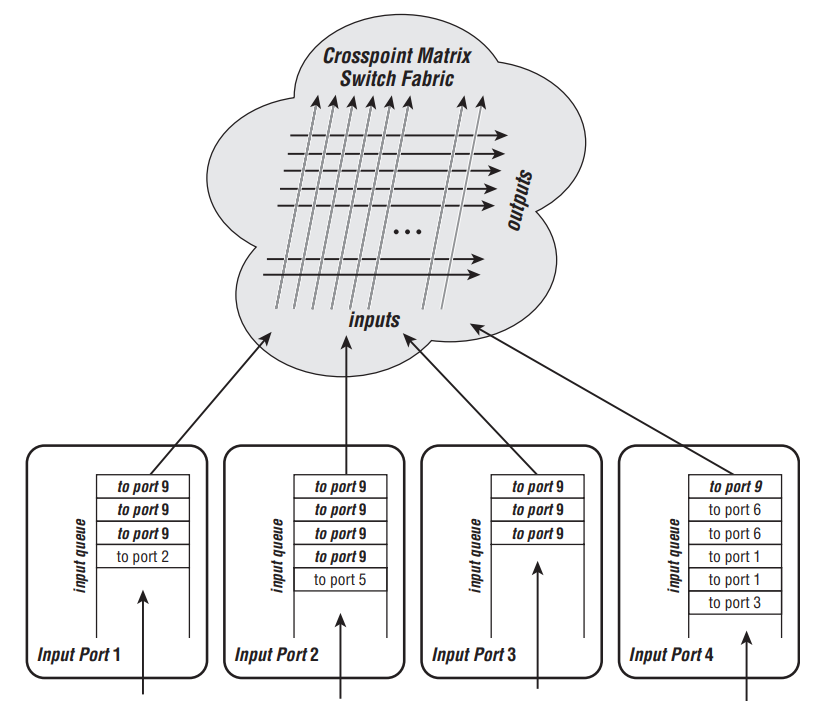
\includegraphics[width=0.9\textwidth]{HOL.png}
  \caption[Headh-of-line blocking]{Head-Of-Line Blocking (fonte: \cite{make})}
  \label{fig:airbus1}
\end{figure}



Na figura 3.3 encontra-se exemplificada uma situação em que as várias tramas do porto 4 não são transmitidas, ainda que os portos de destino das mesmas se encontrem livres. Técnicas que podem ser aplicadas para minimizar ou eliminar as limitações causadas por HOLB incluem equipar os portos com lógica capaz de requerer o envio de tramas que se encontrem em posições mais atrasadas nas filas ou incluir várias filas por porto. \par
Uma forma de contornar as limitações no débtito causados por HOLB é com recurso a OQs (\textit{Output Queue}) ao invés de IQs. Estas funcionam como filas de tramas com destino a um determinado porto. Desse modo, o HOLB desaparece porque a única situação em que uma trama não está a ser transmitida para o porto respetivo é se esse porto já estiver a receber uma outra trama. No entanto, a \textit{switch fabric} necessita de estar preparada para, no pior cenário, transmitir tramas de todos os portos de origem para um mesmo porto de destino, ou seja, o débito nas OQs tem que ser acelerado por um fator equivalente ao número de portos do switch.\par 
Uma opção alternativa é o recurso a VOQs (\textit{Virtual Output Queue}). Esta é uma variante das IQs, na qual, ao invés de haver uma fila em cada porto, há uma fila para cada par de portos origem-destino. De acordo com \cite{VOQ}, VOQs, em conjunto com um algoritmo do tipo \textit{round-robin} para atribuição de permissão de transmissão e recepção de tramas, alcança débitos à saída do switch muito próximos daqueles conseguidos via OQs, sem requerer que a \textit{switch fabric} seja capaz de transferir tramas para um porto com um débito mais elevado do que aquele com que o porto transmite as tramas para os cabos de \textit{Ethernet}. De acordo com \cite{math}, com recurso a uma aceleração por um fator de apenas dois, torna-se possível garantir o mesmo débito que com uma arquitectura com recurso a OQs. \par

